\question{Двудольные графы.}

\begin{definition}
  Двудольный граф это граф, вершины которого могут быть разбиты на два множества
  (две доли) так, что между вершинами каждого из множеств не будет ребер.
\end{definition}

\begin{remark}
  Об обозначениях.

  Двудольный граф обычно обозначается как \(G = \Triple{X, Y, E}\), где \(X\) и
  \(Y\) это его доли, а \(E\)~--- множество ребер между этими долями.

  Пусть задано некоторое подмножество \(S \subseteq X\), тогда \(E(S)\) это
  множество ребер, инцидентных вершинам из множества \(S\).

  Обозначение \(N(S)\) используется что показать 'соседей' для вершин из
  множества \(S\), т.е. такие вершины из множества \(Y\), которые смежны хотя
  бы с одной из вершин из множества \(S\).
\end{remark}

\begin{definition}
  Двудольный граф называется сбалансированным, если размеры его долей совпадают.
\end{definition}

\begin{theorem}\label{bipartite-balance}
  \(r\)-регулярный двудольный граф является сбалансированным.
\end{theorem}
\begin{proof}
  Пусть дан двудольный граф \(G = \Triple{X, Y, E}\).
  Т.к. он двудольный, то множество ребер может быть представлено в виде
  \(\abs{E} = \abs{X} \cdot r\). С другой стороны оно может быть представлено в
  виде \(\abs{E} = \abs{Y} \cdot r\). Приравниваем и получаем искомое равенство
  \(\abs{X} = \abs{Y}\).
\end{proof}

\begin{theorem}
  В любом регулярном двудольном графе существует совершенное паросочетание.
\end{theorem}
\begin{twocolumns}
  \begin{proof}
    Рассмотрим двудольный граф \(G = \Triple{X, Y, E}\). Выберем произвольное
    \(S \subseteq X\). Заметим, что \(E(N(S)) \ge E(S)\), причем т.к. граф
    регулярный, то \(E(N(S)) = \abs{N(S)} \cdot r\), а
    \(E(S) = \abs{S} \cdot r\).

    Подставляя это в полученное ранее неравенство, получаем, что
    \(\abs{N(S)} \ge \abs{S}\) причем это выполняется для любого
    \(S \subseteq X\). Значит по т. Холла (\ref{Hall}) в графе существует
    \(X\)-совершенное паросочетание.

    Т.к. \(G\)~--- регулярный двудольный граф, то по \ref{bipartite-balance} он
    сбалансирован, значит \(\abs{X} = \abs{Y}\). Таким образом \(X\)-совершенное
    паросочетание является совершенным паросочетанием.
  \end{proof}
  \columnbreak

  \begin{figure}[H]
  \centering

  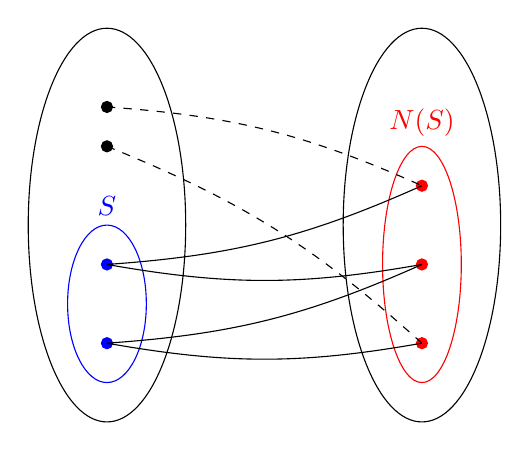
\begin{tikzpicture}
    \coordinate (L1) at (-2, -0.5);
    \coordinate (L2) at (-2, -1.5);

    \coordinate (LS1) at (-2, 1.5);
    \coordinate (LS2) at (-2, 1);

    \coordinate (R1) at (2, 0.5);
    \coordinate (R2) at (2, -0.5);
    \coordinate (R3) at (2, -1.5);

    \draw (-2, 0) ellipse (1cm and 2.5cm);
    \draw (2, 0) ellipse (1cm and 2.5cm);

    \begin{scope}[every path/.style = {color = blue}]
      \draw (-2, -1) ellipse (0.5cm and 1cm);
      \draw node[above] at (-2, 0) {\(S\)};
      \draw[fill = blue] (L1) circle (2pt);
      \draw[fill = blue] (L2) circle (2pt);
    \end{scope}

    \draw[fill = black] (LS1) circle (2pt);
    \draw[fill = black] (LS2) circle (2pt);

    \begin{scope}[every path/.style = {color = red}]
      \draw (2,-0.5) ellipse (0.5cm and 1.5cm);
      \draw node[above] at (2, 1) {\(N(S)\)};
      \draw[fill = red] (R1) circle (2pt);
      \draw[fill = red] (R2) circle (2pt);
      \draw[fill = red] (R3) circle (2pt);
    \end{scope}

    \draw (L1) edge[bend right = 10] (R1);
    \draw (L1) edge[bend right = 10] (R2);
    \draw (L2) edge[bend right = 10] (R2);
    \draw (L2) edge[bend right = 10] (R3);

    \draw[dashed] (LS1) edge[bend left = 10] (R1);
    \draw[dashed] (LS2) edge[bend left = 10] (R3);
  \end{tikzpicture}  
\end{figure}
\end{twocolumns}
